\section{Auswertung}
    \subsection{Die röntgenographische Methode}
        \subsubsection{Gitterkonstante}
            Die verwendete $K_{\alpha}$-Strahlung beinhaltet zwei verschiedene Wellenlängen ($\lambda_{\alpha 1} = 1.5406 \mathring{A}), \lambda_{\alpha 2} = 1.5444 \mathring{A})$,
            daraus wird eine Wellenlänge
            für die Auswertung gemittelt. Die beiden Strahlungen haben ein Intensitätsverhältnis von $\frac{K_{\alpha 2}}{K_{\alpha 1}} = 0.52$
            \begin{align}
                \lambda = \frac{1 \cdot \lambda_{\alpha 1} + 0.52 \cdot \lambda_{\alpha 2}}{1.52}
            \end{align}
            \begin{align*}
                \lambda = 1.5419 \mathring{A}
            \end{align*}

            Aus der Bragg-Bedingung geht hervor, mit $\Psi =  h^2 + l^2 + k^2$ und $d = \frac{a}{\sqrt{\Psi}}$
            \begin{equation}
                n \lambda = 2dsin(\theta) = \frac{2asin(\theta)}{\sqrt{\Psi}} \Leftrightarrow \frac{n \lambda}{2a} = \frac{sin(\theta)}{\sqrt{\Psi}}
            \end{equation}
            Die linke Seite $\frac{n \lambda}{2a}$ ist eine Konstante, da wir $n=1$ annehmen, die Wellenlänge haben wir oben 
            bestimmt und die Gitterkonstante verändert sich nicht bei einer Probe. Der Fundamentalreflex mit dem kleinsten Winkel
            $2\theta$ entspricht nach unserer den Indizes (111), da Reflexe $\leq 3$ in diesem Gitter
            verboten sind. Dadurch können wir auch die 
            weiteren Reflexe finden mit der Relation:
            \begin{align}
                \frac{sin^2(\theta_1)}{\Psi_1} = \frac{sin^2(\theta_2)}{\Psi_2} \\
                \Leftrightarrow \Psi_2 = \frac{sin^2(\theta_2)\Psi_1}{sin^2(\theta_1)}
            \end{align}
            mit $\Psi_1 = 3$ und die Winkel $\theta_{1,2}$ können aus den Messwerten entnommen werden. Theoretisch
            müsste $\Psi_2 \in \mathbb{N}$, durch Messungenauigkeiten stimmt dies nicht ganz. Daher runden wir $\Psi_2$ immer auf die 
            nächste natürliche Zahl. Dieser Zahl kann nun eine Kombination von Indizes zugeordnet werden, da:
            $\Psi_2 = h^2+k^2+l^2$ die Wahl der Indizes ist nicht eindeutig z.B für $\Psi_2 = 2$, würden (110), (011) und (101) passen.
            
            Um daraus nun die Gitterkonstante a zu bestimmen, wird wieder die Bragg-Bedingung genutzt:
            \begin{equation}
                \Leftrightarrow a = \frac{n \lambda \sqrt{\Psi}}{2 sin(\theta)}
            \end{equation}
            wobei $n=1$, $\lambda = 1.54190 \mathring{A}$, $\Psi$ wie oben beschrieben bestimmt und $2 \theta$ wurde gemessen.
            \begin{figure}[H]
                \centering
                \begin{tabular}{c| c| c| c| c}
                    Reflexart & $2 \theta $[\textdegree] & $\Psi_2$ &  mögl. Reflex & a[$\mathring{A}$]\\
                    \hline
                    F & 41.92 & 3 & (111) & 3.733\\
                    F & 48.7 & 4 & (002) & 3.740\\
                    F & 71.36 & 8 & (022) & 3.739\\
                    F & 86.2 & 11 & (113) & 3.742\\
                    F & 91.02 & 12 & (222) & 3.744\\
                    Ü & 23.84 & 1 & (001) & 3.733\\
                    Ü & 33.96 & 2 & (011) & 3.733\\
                    Ü & 54.8 & 5 & (012) & 3.746\\
                    Ü & 60.5 & 6 & (112) & 3.749\\
                    Ü & 76 & 9 & (122) & 3.757\\
                    Ü & 81.56 & 10 & (013) & 3.733\\
                    Ü & 96.26 & 13 & (023) & 3.733\\
                    Ü & 100.76 & 14 & (123) & 3.745\\
                \end{tabular}
                \caption{Gitterkonstanten Probe 2}
            \end{figure}
            
            \begin{figure}[H]
                \centering
                \centering
                \begin{tabular}{c | c | c | c | c}
                    Reflexart & $2 \theta $[\textdegree] & $\Psi_2$ &  mögl. Reflex & a[$\mathring{A}$]\\
                    \hline
                    F & 41.06 & 3 & (111) & 3.808\\
                    F & 47.86 & 4 & (002) & 3.801\\
                    F & 71.08 & 8 & (022) & 3.751\\
                    F & 85.98 & 11 & (113) & 3.750\\
                    F & 90.5 & 12 & (222) & 3.760\\
                    Ü & 23.5 & 1 & (001) & 3.786\\
                    Ü & 33.74 & 2 & (011) & 3.757\\
                    Ü & 54.6 & 5 & (012) & 3.759\\
                    Ü & 60.3 & 6 & (112) & 3.760\\
                    Ü & 76 & 9 & (122) & 3.757\\
                    Ü & 95.76 & 13 & (023) & 3.748\\
                    Ü & 100.5 & 14 & (123) & 3.752\\
                \end{tabular}
                \caption{Gitterkonstanten Probe 3}
            \end{figure}
            
            \begin{figure}[H]
                \centering
                \begin{tabular}{c | c | c | c | c}
                    Reflexart & $2 \theta $[\textdegree] & $\Psi_2$ &  mögl. Reflex & a[$\mathring{A}$]\\
                    \hline
                    F & 40.46 & 3 & (111) & 3.862\\
                    F & 47.08 & 4 & (002) & 3.861\\
                    F & 68.88 & 8 & (022) & 3.856\\
                    F & 82.9 & 11 & (113) & 3.863\\
                    F & 87.6 & 12 & (222) & 3.859\\
                \end{tabular}
                \caption{Gitterkonstanten Probe 4}
            \end{figure}

            Für jede Probe wird jetzt der Mittelwert der Gitterkonstante mit zugehörigem
            Fehler berechnet, nach den Formeln:
            \begin{equation}
                \bar{a} = \frac{1}{n} \sum^n_i a_i
            \end{equation}
            \begin{equation}
                \Delta \bar{a} = \sqrt{\frac{1}{n(n-1)} \sum^n_i (\bar{a}-a_i)^2}
            \end{equation}  
            es ergibt sich:
            \begin{align*}
                \bar{a}_{Probe2} = (3,74 \pm 0,002)[\mathring{A}]\\
                \bar{a}_{Probe3} = (3,77 \pm 0,006)[\mathring{A}]\\
                \bar{a}_{Probe4} = (3,86 \pm 0,001)[\mathring{A}]
            \end{align*}
            Im Anhang befinden sich unsere Röntgendiffraktogramme und die dazu gefitteten Gaußpeaks.
            Probe 2: \ref{Röntgendiffraktogramm Probe 2}, Probe 3: \ref{Röntgendiffraktogramm Probe 3}, Probe 4: \ref{Röntgendiffraktogramm Probe 4}

            \subsubsection{Bestimmung des Ordnungsgrades}
                Um den Ordnungsgrad der Proben zu bestimmen nutzen wir die Formel:
                \begin{equation}
                    S^2 = \frac{I^{\text{Ü}}}{I^F}(\frac{(f_{Au}+3f_{Cu})^F}{(f_{Au}-f_{Cu})^{\text{Ü}}})^2 \frac{(pL_p)^F}{(pL_p)^\text{Ü}}
                    %S^2 = \frac{I^Ü}{I^F} (\frac{(f_{Au} + 3 f_{Cu})^F}{(f_{Au}-f_{Cu})^Ü})^2 \frac{(pL_p)^F)}{(pL_p)^Ü}
                \end{equation}

                %mit dem Lorentz-Polarisationsfaktor L_p \eqref{Lorentz-Polarisationsfaktor}

                Beim bestimmen der Intensität musste darauf geachtet werden, dass das Untergrundrauschen 
                möglichst gut entfernt wird. Dazu haben wir probiert den Untergrund mit einem 
                Fit zu beschreiben, und diesen dann von den Messwerten abzuziehen. Um die Intensität
                nun zu berechnen, haben wir über die Gaußkurven der Peaks integriert. Den Flächenhäufigkeitsfaktor
                kann man aus folgender Tabelle der Anleitung für die möglichen Reflexe ablesen.
                Da man das Verhältnis eines Überstrukturreflexes und einem Fundamentalreflex betrachtet,
                entfällt der zweite Korrekturterm (Absorbtionsfaktor). Die Atomformfaktoren haben wir 
                mit Hilfe der Tablle und Formel aus der Anleitung bestimmt.

                \begin{figure}
                    \centering
                    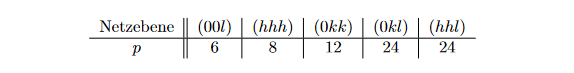
\includegraphics{images/flächenhäufigkeitsfaktor.PNG}
                    \caption{Flächenhäufigkeitsfaktor}
                \end{figure}

                \begin{figure}[H]
                    \centering
                    \begin{tabular}{c | c | c | c | c | c | c}
                        Intensität & $2\theta$ & $f_{Cu}$ & $f_{Au}$ & p & $L_p$ & $S^2$\\
                        \hline
                        199 & 23.84 & 72.66 & 25.93 & 6 & 5.5 & 0.33\\
                        70 & 33.96 & 68.14 & 23.93 & 12 & 2.587 & 0.14\\
                        1868 & 41.92 & 64.66 & 22.36 & 8 & 1.625 & -\\
                        1646 & 48.7 & 61.87 & 21.06 & 6 & 1.159 & -\\
                        89 & 54.8 & 59.53 & 19.93 & 24 & 0.886 & 0.18\\
                        89 & 60.5 & 57.49 & 18.93 & 24 & 0.708 & 0.46\\
                        514 & 71.36 & 53.98 & 17.19 & 12 & 0.499 & -\\
                        69 & 76 & 52.64 & 16.53 & 24 & 0.443 & 0.65\\
                        79 & 81.56 & 51.15 & 15.79 & 24 & 0.395 & 0.66\\
                        814 & 86.2 & 50.00 & 15.22 & 24 & 0.368 & -\\
                        176 & 91.02 & 48.89 & 14.68 & 8 & 0.351 & -\\
                        59 & 96.26 & 47.79 & 14.14 & 24 & 0.342 & 0.87\\
                        74 & 100.76 & 46.91 & 13.72 & 0 & 0.342 & -\\
                    \end{tabular}
                    \caption{Ordnungsgrad Probe 2}
                \end{figure}

                \begin{figure}[H]
                    \centering
                    \begin{tabular}{c | c | c | c | c | c | c}
                        Intensität & $2\theta$ & $f_{Cu}$ & $f_{Au}$ & p & $L_p$ & $S^2$\\
                        \hline
                        104 & 23.5 & 72.81 & 26 & 6 & 5.668 & 0.137\\
                        50 & 33.74 & 68.23 & 23.97 & 12 & 2.624 & 0.080\\
                        2437 & 41.06 & 65.02 & 22.53 & 8 & 1.702 & - \\
                        1334 & 47.86 & 62.21 & 21.22 & 6 & 1.205 & - \\
                        37 & 54.6 & 59.6 & 19.97 & 24 & 0.89 & 0.094\\
                        40 & 60.3 & 57.56 & 18.96 & 24 & 0.714 & 0.188\\
                        564 & 71.08 & 54.07 & 17.24 & 12 & 0.502 & - \\
                        44 & 76 & 52.64 & 16.53 & 24 & 0.443 & 0.380\\
                        575 & 85.98 & 50.05 & 15.25 & 24 & 0.369 &  -\\
                        89 & 90.5 & 49.01 & 14.74 & 8 & 0.352 &  -\\
                        49 & 95.76 & 47.89 & 14.19 & 24 & 0.342 & 1.445\\
                        79 & 100.5 & 46.96 & 13.75 & 0 & 0.342 & - \\
                    \end{tabular}
                    \caption{Ordnungsgrad Probe 3}
                \end{figure}

                Aus diesen Werten wird der mittlere Ordnungsgrad mit Fehler, wie schon bei der Gitterkonstanten, 
                bestimmt:
                \begin{align}
                    \bar{S_2} = 0.47 \pm 0.09\\
                    \bar{S_3} = 0.39 \pm 0.22
                \end{align}

                In den beiden Tabellen gibt es zwei Auffälligkeiten. Bei den Winkeln $\approx 100$°
                ist $\Psi_2 = 14$, welches keinem Flächenhäufigkeitsfaktor zugeordnet werden kann. Daher fallen
                die beiden Werte bei unserer Berechnung raus. Was außerdem auffällt ist, dass bei der Probe 3 
                der Ordnungsgrad des Winkels $95,76$° größer als 1 ist. Da $0 \leq S \leq 1$ sein muss, ist dies 
                vermutlich ein Messfehler.
            


